\section{Hitting Probabilities and Absorption Times}\label{section: hitting probabilities and hitting times}
Let $X_0, X_1, \dots$ be a Markov chain on a finite state space $V$, 
and let $\P_v$ denote the law of the Markov chain initialized at state $v$, 
or in other words $X_0 = v$.
Define $T_u$ to be the \textbf{hitting time} of vertex $u$ by the Markov chain,
given by
\begin{align*}
    T_u = \min\{t \geq 0: X_t = u\},
\end{align*}
where if no such $t$ exists then $T_u = \infty$.

For an absorbing Markov chain, 
let the set of absorbing states be $U \subseteq V$.
If our starting vertex $v$ belongs to $U$, then the behavior of the chain is trivial,
so we will assume henceforth that $v \not\in U$.
We define the \textbf{hitting probability} of $u \in U$ by
\begin{align*}
    h_u(v) = \P_v (\mbox{$X_t = u$ for all $t$ sufficiently large}),
\end{align*}
where $\P_v$ denotes the law of the Markov chain initiated at $v$.
The hitting probability is equivalently
\begin{align*}
    h_u(v) = \P_v (\forall u' \in U,\,\, T_u \leq T_{u'} ),
\end{align*}
which will give us the flexibility later on to modify the Markov chain so that the states in $U$ are no longer absorbing.
As an absorbing Markov chain reaches an absorbing state with probability 1,
for any $v$ we have
\begin{align*}
    \sum_{u \in U} h_u(v) = 1.
\end{align*}
% Also notice that if $u' \in U$ we have $h_u(u')=1$ if $u'=u$ and $h_u(u')=0$ otherwise.

In order to measure hitting probabilities $h_{u}(v)$ 
through the hunger game process, 
we consider a modification of the Markov chain
in which all absorbing states go to $v$ with probability 1.
In other words, for each $u\in U$ we replace $P_u$, the row of $P$ corresponding to state $u$, with $e_v$, the unit vector corresponding to $v$.
Crucially, this modification does not change 
the hitting probabilities $h_{u}(v)$
as given by our second definition.
Additionally, we remove any states in $V$ 
that cannot be reached from $v$ with positive probability;
this does not alter the hitting probabilities.
We will refer to this modified Markov chain as the 
\textbf{rerouted Markov chain} associated with $v$.
Due to the removal of unreachable states, a rerouted Markov chain of an absorbing Markov chain is always irreducible.

\begin{example}\label{example: rerouted MC}
Consider the absorbing Markov chain given in \cref{subfig: ex rerouted base}\,, 
which has absorbing states $v_1$ and $v_4$.
\begin{figure}[htbp]
    \centering
    \begin{subfigure}{\textwidth}
        \centering
        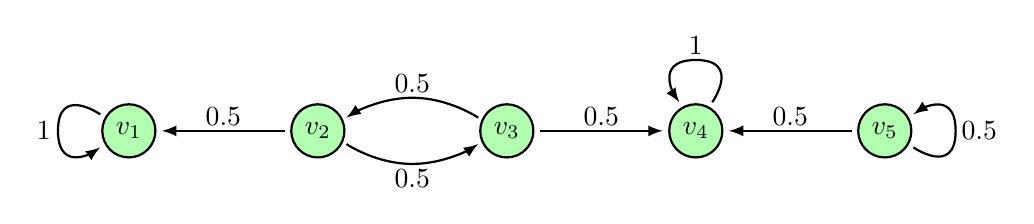
\begin{tikzpicture}[scale=0.6,font=\normalsize,baseline,thick]
            \foreach \x in {1,...,5} {
                \filldraw[color=black,fill=green!30,thick] (4*\x,0) circle (16pt);
                \node at (4*\x,0) {$v_{\x}$};
            }
            \draw [->,>=latex] plot [smooth,tension=5] coordinates {(4-0.866*0.7,0.5*0.7) (4-1.5,0) (4-0.866*0.7,-0.5*0.7)};
            \node at (2.2,0) {1};
            \draw[->,>=latex] (4*2-0.7,0) -- (4*1+0.7,0);
            \node at (4*1+2,0.3) {0.5};
            \draw [->,>=latex] plot [smooth,tension=1] coordinates {(4*3-0.866*0.7,0.4*0.7) (4*3-2,0.7) (4*3-4+0.866*0.7,0.4*0.7)};
            \node at (4*3-2,1) {0.5};
            \draw [->,>=latex] plot [smooth,tension=1] coordinates {(4*2+0.866*0.7,-0.4*0.7) (4*2+2,-0.7) (4*2+4-0.866*0.7,-0.4*0.7)};
            \node at (4*2+2,-1) {0.5};
            \draw[->,>=latex] (4*3+0.7,0) -- (4*4-0.7,0);
            \node at (4*3+2,0.3) {0.5};
            \draw [->,>=latex] plot [smooth,tension=5] coordinates {(4*4+0.5*0.7,0.866*0.7) (4*4+0,1.5) (4*4-0.5*0.7,0.866*0.7)};
            \node at (4*4,1.8) {1};
            \draw[->,>=latex] (4*5-0.7,0) -- (4*4+0.7,0);
            \node at (4*5-2,0.3) {0.5};
            \draw [->,>=latex] plot [smooth,tension=5] coordinates {(4*5+0.866*0.7,-0.5*0.7) (4*5+1.5,0) (4*5+0.866*0.7,0.5*0.7)};
            \node at (22,0) {0.5};
        \end{tikzpicture}
        \caption{An absorbing Markov chain.}
        \label{subfig: ex rerouted base}
    \end{subfigure}
    \begin{subfigure}{\textwidth}
        \centering
        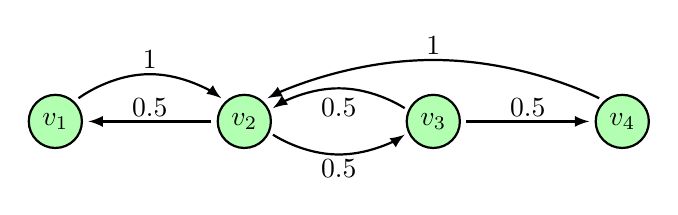
\begin{tikzpicture}[scale=0.6,font=\normalsize,baseline,thick]
            \foreach \x in {1,...,4} {
                \filldraw[color=black,fill=green!30,thick] (4*\x,0) circle (16pt);
                \node at (4*\x,0) {$v_{\x}$};
            }
            \draw [->,>=latex] plot [smooth,tension=1] coordinates {(4*1+0.7*0.7,0.7*0.7) (4*2-2,1) (4*2-0.7*0.7,0.7*0.7)};
            \node at (4*1+2,1.3) {1};
            \draw[->,>=latex] (4*2-0.7,0) -- (4*1+0.7,0);
            \node at (4*1+2,0.3) {0.5};
            \draw [->,>=latex] plot [smooth,tension=1] coordinates {(4*3-0.866*0.7,0.4*0.7) (4*3-2,0.7) (4*3-4+0.866*0.7,0.4*0.7)};
            \node at (4*3-2,0.3) {0.5};
            \draw [->,>=latex] plot [smooth,tension=1] coordinates {(4*2+0.866*0.7,-0.4*0.7) (4*2+2,-0.7) (4*2+4-0.866*0.7,-0.4*0.7)};
            \node at (4*2+2,-1) {0.5};
            \draw[->,>=latex] (4*3+0.7,0) -- (4*4-0.7,0);
            \node at (4*3+2,0.3) {0.5};
            \draw [->,>=latex] plot [smooth,tension=1] coordinates {(4*4-0.7*0.7,0.7*0.7) (4*3,1.3) (4*2+0.7*0.7,0.7*0.7)};
            \node at (4*3,1.6) {1};
        \end{tikzpicture}
        \caption{The rerouted Markov chain associated with $v_2$.}
        \label{subfig: ex rerouted 2}
    \end{subfigure}
    \caption{A rerouted Markov chain.}
    \label{fig: ex rerouted}
\end{figure}
The rerouted Markov chain associated with non-absorbing state $v_2$ 
is shown in \cref{subfig: ex rerouted 2}\,, 
where since $v_5$ cannot reach $v_2$ with positive probability, 
it is removed from the system; this ensures that the Markov chain is irreducible.
Hence, it has a unique stationary distribution; this applies for all rerouted Markov chains of any finite absorbing Markov chain.
\end{example}

The following lemma will be useful for the upcoming result, \cref{theorem: hitting probability absorbing}.

\begin{lemma}\label{lemma: hitting probability absorbing helper deviation}
Let $a$ and $b$ be positive real numbers and let $a'$ and $b'$
be nonnegative real numbers.
For a given $\varepsilon$ satisfying $0 \leq \varepsilon < \frac{a+b}{2}$,
if $\left|a'-a\right|\leq \varepsilon$ and
$\left|b'-b\right| \leq \varepsilon$, then
\begin{align*}
    \frac{a-\varepsilon}{a+b} \leq \frac{a'}{a'+b'}
    \leq \frac{a+\varepsilon}{a+b}.
\end{align*}
\end{lemma}
\begin{proof}
Let $a'=a+\delta_1$ and $b'=b+\delta_2$,
where $|\delta_1|,|\delta_2| \leq \varepsilon$.
First, notice that $\frac{a'}{a'+b'}$ is well-defined,
as $a'+b' = a+b+\delta_1+\delta_2 \geq a+b-2\varepsilon > 0$.
Since $a' \geq 0$, $\frac{a'}{a'+b'}\geq 0$.
Holding $a$ and $b$ fixed, we see that the quantity 
$\frac{a'}{a'+b'} = 1/(1+\frac{b'}{a'})
= 1/(1+\frac{b+\delta_2}{a+\delta_1})$
is weakly increasing with respect to $\delta_1$
and weakly decreasing with respect to $\delta_2$.
(Technically this argument requires $a+\delta_1 > 0$
and therefore does not handle the case $a'=0$
but this case is easily dealt with separately.)
Hence, within the bounds for $\delta_1$ and $\delta_2$,
$\frac{a'}{a'+b'}$ is minimized
when $\delta_1 = -\varepsilon$ and $\delta_2 = \varepsilon$, yielding
\begin{align*}
    \frac{a'}{a'+b'}
    = \frac{a+\delta_1}{a+b+\delta_1+\delta_2}
    \geq \frac{a-\varepsilon}{a+b-\varepsilon+\varepsilon}
    = \frac{a-\varepsilon}{a+b},
\end{align*}
and $\frac{a'}{a'+b'}$ is maximized
when $\delta_1 = \varepsilon$ and $\delta_2 = -\varepsilon$, yielding
\begin{align*}
    \frac{a'}{a'+b'}
    = \frac{a+\delta_1}{a+b+\delta_1+\delta_2}
    \leq \frac{a+\varepsilon}{a+b+\varepsilon-\varepsilon}
    = \frac{a+\varepsilon}{a+b},
\end{align*}
which completes the proof.
\end{proof}

The following theorem demonstrates how 
the hitting probabilities of a finite absorbing Markov chain 
are approximated by the firing vector of the rerouted Markov chain.

\begin{theorem}\label{theorem: hitting probability absorbing}
Given a finite absorbing Markov chain, let $\v^{(N)}$ be the firing vector 
after $N$ steps of a hunger game process 
on the rerouted Markov chain associated with state $v$.
Then the sequence $\{a_N\}$ defined by
\begin{align*}
    a_N = \frac{\v^{(N)}_u}{\displaystyle\sum_{u' \in U} \v^{(N)}_{u'}},
\end{align*}
where we define $a_N$ to be 0 when the denominator equals 0, 
converges to the hitting probability $h_u(v)$ with discrepancy $O(1/N)$; 
that is, there exists a constant $C$ such that 
$a_N$ differs from $h_u(v)$ by at most $\frac{C}{N}$ for all $N$. 
\end{theorem}
\begin{proof}
In the rerouted Markov chain, 
$v$ can reach every state in $V$, and every state in $V$ 
can reach an absorbing state (as the original Markov chain was absorbing), 
which in the rerouted Markov chain moves back to $v$ with probability 1; 
as a result, the rerouted Markov chain is irreducible.
By \cref{theorem: irreducible fidelity converge stationary}\,,
the normalized firing vector $\frac{1}{N}\v^{(N)}$ 
converges to the unique stationary distribution $\ppi$ 
of the rerouted Markov chain within distance $\frac{c}{N}$ 
for some constant $c$.

It is a standard fact that the expected number of visits to state $w$ 
before returning to $v$ is given by $\frac{\ppi_w}{\ppi_v}$; 
see, for example, \cite[Theorem 1.7.6]{norris1998markov}.
But, as after visiting some $u'\in U$ the next state visited must be $v$,
meaning $u'$ can be visited at most once before returning to $v$,
the expected number of visits to any such $u'$ 
equals the probability of visiting $u'$ before returning to $v$.
As a result, for all $u \in U$, the hitting probability $h_{u}(v)$ 
is proportional to $\ppi_{u}$, and given that an absorbing Markov chain 
reaches an absorbing state with probability 1, we have
\begin{align*}
    h_{u}(v) = \frac{\ppi_{u}}{\displaystyle\sum_{u' \in U} \ppi_{u'}}.
\end{align*}

As $\sum_{u' \in U} \ppi_{u'}$ is a positive constant, 
there exists a finite $M$ such that for all $N>M$ we have
\begin{align*}
    \frac{c}{N} < \frac{1}{2} \sum_{u' \in U} \ppi_{u'}
\end{align*}
with $c$ as above.
As $a_N \in [0,1]$ is bounded, there exists a constant $C_1$ 
such that $a_N$ is within $\frac{C_1}{N}$ of $h_u(v)\in[0,1]$ for all $N \leq M$;
in particular, $C_1=M$ suffices.

For $N > M$, notice that
\begin{align*}
    a_N = \dfrac{\v_u^{(N)}}{\displaystyle\sum_{u'\in U} \v_{u'}^{(N)}}
    = \dfrac{\frac{1}{N}\v_u^{(N)}}{\frac{1}{N}\v_u^{(N)} + {\displaystyle\sum_{u'\in U\setminus\{u\}}} \frac{1}{N} \v_{u'}^{(N)}}.
\end{align*}
As $\frac{1}{N}\v^{(N)}$ is within distance $\frac{c}{N}$ of $\ppi$ in the $L^1$ metric, we know both $\left|\frac{1}{N}\v_u^{(N)}-\ppi_u\right| \leq \frac{c}{N}$ and
\begin{align*}
    \left|\displaystyle\sum_{u'\in U\setminus\{u\}}\frac{1}{N} \v_{u'}^{(N)} - \displaystyle\sum_{u' \in U\setminus\{u\}} \ppi_{u'}\right| \leq \frac{c}{N}.
\end{align*}
Due to the rerouted Markov chain being irreducible, we also know that $\ppi_v > 0$ for all states $v\in V$; in addition, each component of the visit vector $\v^{(N)}$ is a nonnegative integer.
Lastly, by definition of $M$, we have
\begin{align*}
    0 \leq \frac{c}{N} < \frac{1}{2} \left(\ppi_{u} + \sum_{u'\in U\setminus\{u\}} \ppi_{u'}\right).
\end{align*}
Letting $\varepsilon = \frac{c}{N}$, we apply
\cref{lemma: hitting probability absorbing helper deviation} with the values
\begin{align*}
    a = \ppi_u > 0, \qquad\quad
    b = \sum_{u'\in U\setminus\{u\}} \ppi_{u'} > 0, \qquad\quad
    a' = \frac{1}{N}\v_u^{(N)} \geq 0, \qquad\quad
    b' = \sum_{u'\in U\setminus\{u\}}\frac{1}{N} \v_{u'}^{(N)} \geq 0
\end{align*}
to find
\begin{align*}
    \frac{\ppi_{u} - \frac{c}{N}}{\ppi_{u} + \displaystyle\sum_{u'\in U\setminus\{u\}} \ppi_{u'}}
    \leq \dfrac{\frac{1}{N}\v_u^{(N)}}{\frac{1}{N}\v_u^{(N)} + {\displaystyle\sum_{u'\in U\setminus\{u\}}} \frac{1}{N} \v_{u'}^{(N)}}
    \leq \frac{\ppi_u + \frac{c}{N}}{\ppi_{u} + \displaystyle\sum_{u'\in U\setminus\{u\}} \ppi_{u'}},
\end{align*}
or equivalently
\begin{align*}
    h_u(v) - \frac{1}{N}\cdot\frac{c}{\displaystyle\sum_{u'\in U}\ppi_{u'}}
    \leq a_N
    \leq h_u(v) + \frac{1}{N}\cdot\frac{c}{\displaystyle\sum_{u'\in U}\ppi_{u'}}.
\end{align*}

Thus, the deviation of $a_N$ from $h_u(v)$ is at most
\begin{align*}
    \dfrac{1}{N}\cdot\frac{c}{\displaystyle\sum_{u' \in U} \ppi_{u'}}.
\end{align*}
The second factor is a constant, which we will denote $C_2$, 
and thus taking $C=\max(C_1,C_2)$ 
we find that for all $N$, $a_N$ differs from $h_u(v)$ by at most $\frac{C}{N}$.
\end{proof}

\begin{remark}\label{remark: escape probability}
We can apply \cref{theorem: hitting probability absorbing} 
to deterministically approximate the escape probability of $u$ from $v$ 
on an irreducible Markov chain, or the probability that a chain 
starting at state $v$ reaches state $u$ before returning to $v$.
We do this by splitting vertex $v$ into vertices $v_0$ and $v_1$ 
where all outgoing edges of $v$ now emanate from $v_0$ 
and all inbound edges of $v$ now end at $v_1$.
Furthermore, we may remove all outgoing edges from vertex $u$.
The resulting Markov chain is absorbing 
with the set of absorbing states $U=\{u,v\}$, 
and thus one may use \cref{theorem: hitting probability absorbing} 
on the rerouted Markov chain associated with state $v_0$ 
to approximate the hitting probability $h_{v_1}(v_0)$.
Notice that $h_{v_1}(v_0)$ equals the escape probability 
of $u$ from $v$ in the original irreducible Markov chain, 
and thus \cref{theorem: hitting probability absorbing} 
enables us to calculate escape probabilities.
\end{remark}

We now consider the \textbf{absorption time} of an absorbing Markov chain
whose set of absorbing states is $U \subseteq V$, given by
\begin{align*}
    T_U = \min\{t \geq 0: X_t \in U\}.
\end{align*}
At the absorption time, the chain enters an absorbing state, 
where it remains forever.

For example, starting at state $v_2$ in the absorbing Markov chain given in \cref{subfig: ex rerouted base}, with probability $\frac{1}{2}$ we enter absorbing state $v_1$ in the first step, and otherwise move to state $v_3$, which has the same 50-50 split between moving to an absorbing state ($v_4$) or not ($v_2$).
Thus $T_U$ in this case is a geometric random variable with success probability $\frac{1}{2}$, which has expected value 2.

The expected absorption time is $\E_v T_U$, 
where $\E_v$ denotes the expected value for the law 
of the Markov chain initialized at state $v$.
Then, when using the rerouted Markov chain, 
a chain can naturally be divided into epochs 
each of which ends with an occurrence of a state in $U$, 
which is then rerouted in the next time step to $v$.
Hence, the expected absorption time $\E_v T_U$ 
can be calculated from the stationary distribution $\ppi$ 
of the rerouted Markov chain associated with $v$ to be
\begin{align*}
    \E_v T_U = \frac{1}{\displaystyle\sum_{u \in U} \ppi_u}-1.
\end{align*}
Notice that if $v \in U$, then $\E_v T_U = 0=\frac{1}{1}-1$; 
the $-1$ term corresponds to the extra time step needed to reroute 
from an absorbing state to $v$ for each epoch.

The following theorem shows how the expected absorption time 
of an absorbing Markov chain can be approximated 
using the normalized firing vector of the rerouted Markov chain.

\begin{theorem}\label{theorem: absorption time}
Given an absorbing Markov chain, let $\v^{(N)}$ be the firing vector 
after $N$ steps of the hunger game process on the rerouted Markov chain 
associated with state $v$.
Then the sequence $\{b_N\}$ defined by
\begin{align*}
    b_N = \frac{N}{\displaystyle\sum_{u \in U} \v^{(N)}_u}-1,
\end{align*}
where we define $b_N$ to be 0 when the denominator equals 0, 
converges to the expected absorption time $\E_v T_U$, 
where there exists a constant $C$ such that $b_N$ 
is within distance $\frac{C}{N}$ of $\E_v T_U$ for all $N$.
\end{theorem}
\begin{proof}
From the proof of \cref{theorem: hitting probability absorbing}\,,
we see that the rerouted Markov chain 
has a unique stationary distribution $\ppi$, and thus 
the normalized firing vector $\frac{1}{N}\v^{(N)}$ 
converges to $\ppi$ within distance $\frac{c}{N}$ for some constant $c$.

As $\sum_{u \in U} \ppi_{u}$ is a positive constant, 
there exists a finite $M$ such that for all $N>M$ we have
\begin{align*}
    \frac{c}{N} < \frac{1}{2} \sum_{u \in U} \ppi_{u}.
\end{align*}
As $b_N$ is finite, there exists a constant $C_1$ 
such that $b_N$ is within $\frac{C_1}{N}$ of $\E_v T_U$ for all $N \leq M$.
For $N > M$, it suffices to show the existence of a constant $C_2$ 
such that for all $N > M$,
\begin{align*}
    \left| \frac{1}{\displaystyle\sum_{u \in U} \frac{1}{N}\v^{(N)}_u} - \frac{1}{\displaystyle\sum_{u \in U} \ppi_u} \right| < \frac{C_2}{N}. 
\end{align*}
The furthest away $b_N$ can be from $\E_v T_U$ 
results in the left hand side becoming
\begin{align*}
    \frac{1}{-\displaystyle\frac{c}{N} + \displaystyle\sum_{u \in U} \ppi_u} - \frac{1}{\displaystyle\sum_{u \in U} \ppi_u} = \frac{1}{N}\cdot\frac{c}{\left(-\displaystyle\frac{c}{N} + \displaystyle\sum_{u \in U} \ppi_u\right)\left(\displaystyle\sum_{u \in U} \ppi_u\right)}.
\end{align*}
As $N>M$, we have
\begin{align*}
    -\frac{c}{N}+\displaystyle\sum_{u \in U} \ppi_{u} > \frac{1}{2}\sum_{u \in U} \ppi_{u} > 0,
\end{align*}
so in the worst case the deviation from $\E_v T_U$ is less than
\begin{align*}
    \frac{1}{N}\cdot \frac{2c}{\left(\displaystyle\sum_{u \in U} \ppi_{u}\right)^2}.
\end{align*}
The second factor is a constant, which we will denote $C_2$, 
and thus taking $C=\max(C_1,C_2)$ yields that $b_N$ 
is at most $\frac{C}{N}$ away from $\E_v T_U$ for all $N$.
\end{proof}

\begin{remark}\label{remark: expected return time irreducible}
We can apply \cref{theorem: absorption time} to calculate 
the expected return time for state $v$ in an irreducible Markov chain.
We do this in a similar method to \cref{remark: escape probability} 
by splitting vertex $v$ into vertices $v_0$ and $v_1$ 
where all outgoing edges of $v$ now emanate from $v_0$ 
and all inbound edges of $v$ now end at $v_1$.
The resulting Markov chain is absorbing with unique absorbing state $v_1$, 
and thus one may use \cref{theorem: absorption time} 
on the rerouted Markov chain associated with state $v_0$ 
to approximate the expected absorption time.
As $v_1$ is the only absorbing state, this calculates 
the expected hitting time from $v_0$ to $v_1$, 
which is the expected return time from $v$ 
in the original irreducible Markov chain.
\end{remark}
